\documentclass{article}
\usepackage[utf8]{inputenc}
\usepackage{graphicx}
\usepackage{epstopdf}
\usepackage{caption}
\usepackage{subcaption}
\usepackage{multirow}
\usepackage{hyperref}
\usepackage{url}
\usepackage{seqsplit}
\hypersetup{pdfstartview={FitH null null null}}
\usepackage{amssymb,amsmath}
\usepackage{amsthm}
\usepackage{empheq}
\usepackage{algorithm,algpseudocode}
\usepackage[margin=1.5in]{geometry}
\usepackage{listings}
\lstset{language=Python} 

\usepackage{listings}
\usepackage{color} %red, green, blue, yellow, cyan, magenta, black, white
\definecolor{mygreen}{RGB}{28,172,0} % color values Red, Green, Blue
\definecolor{mylilas}{RGB}{170,55,241}


\title{Ab-initio modeling using a fragment matching and energy functions}
\author{Caiwei Wang, Xiaokai Qian, Sean Lander, Haipei Fan, Puneet Gaddam, Brett Koonce\\University of Missouri - Columbia}

\date{March 10, 2013}

\algloopdefx{NoEndIf}[1]{\textbf{If} #1 \textbf{then}}

\begin{document}

\maketitle

\section{Abstract}
This project is to develop a simple prototype of fragment assembly template-free modeling system. First, we convert PDB into residue-torsion pairs and use sliding window along to get lists for building fragment database created by Rosetta. Next, we can randomly select from list of matches. After initialization, we use simulated annealing to judge if the fragment’s neighbor can be accepted according to consensus scoring. Finally, we can get millions of decoys that are scored and sorted for evaluation. Ultimately, we create a movie of the top-scoring protein.

\section{Introduction}

Template free modeling is an important technique in modern bioinformatics since not all proteins have templates. First, we begin with PDB sequences converting into torsion angles using rama/lipa. By sliding window algorithm, we can get millions of fragments to construct the database. Then for each segment do a query for a complete match in the database.\\\\
We use simulated annealing to score, when the current solution’s neighbor is better, accepted. If not, we select it with a probability based on the current temperature. We modified consensus scoring for model acceptance. If the score improves for 2/3 through the scoring techniques D-fire energy function, accepted. Otherwise, do normalization and sum to be accepted upon temperature based probability.\\\\
For our project, we implemented basic homology modeling in python 3.3, using a number of external tools like D-fire, Rosetta, TM-score presenting a final visualized model.


\subsection{Pipeline}
\begin{figure}[H]
\begin{center}
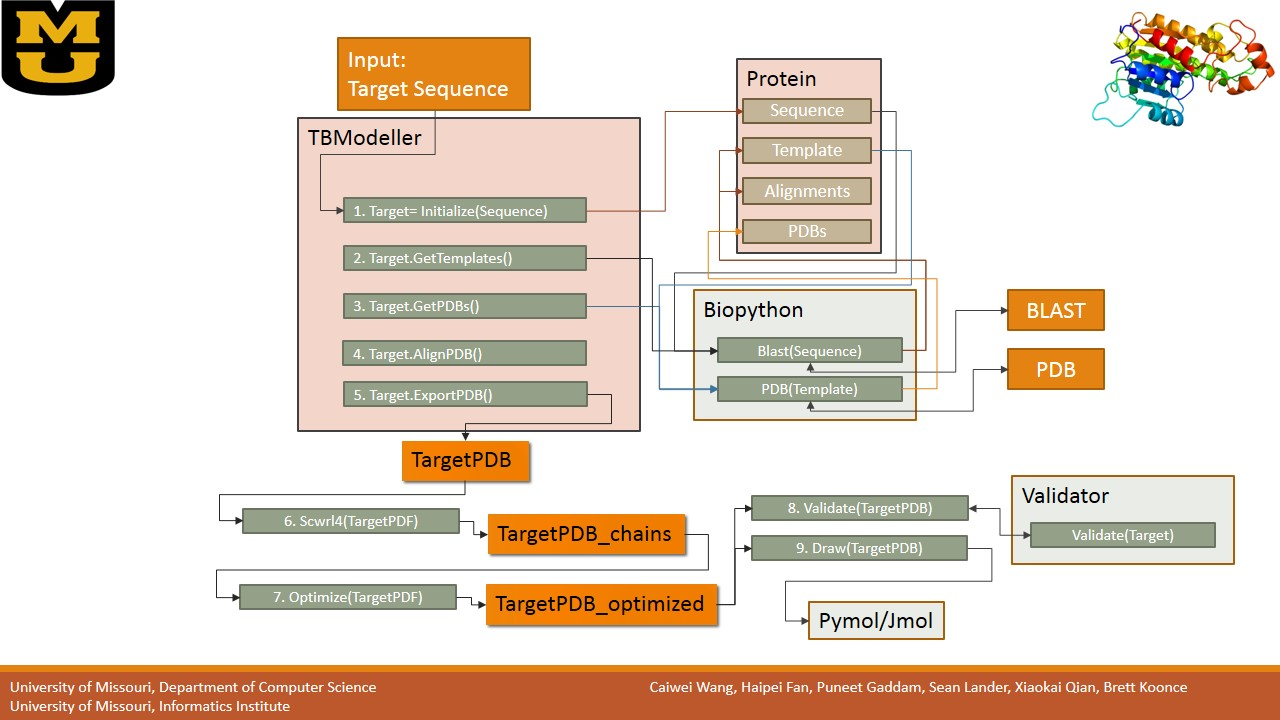
\includegraphics[width=\textwidth]{workflow}
\caption{An overview of the TBPy pipeline}
\label{Fig:blosum}
\end{center}
\end{figure}

\section{Target goal}

\subsection{CASP}

\section{Fragment database}

\section{Simulated annealing}

\subsection{d-DFIRE score}

\subsection{BLOSUM62 selection}


\section{Results/statistics}


\newpage
\section{Visualization}

After we obtain our final target PDB file, we use Jmol to visualize it. At the same time, we also visualize the native one to compare it with our prediction.  The left one is a target structure we generated (T0644), while right one is the native structure.

\begin{figure}
\centering
\begin{minipage}{.5\textwidth}
  \centering
  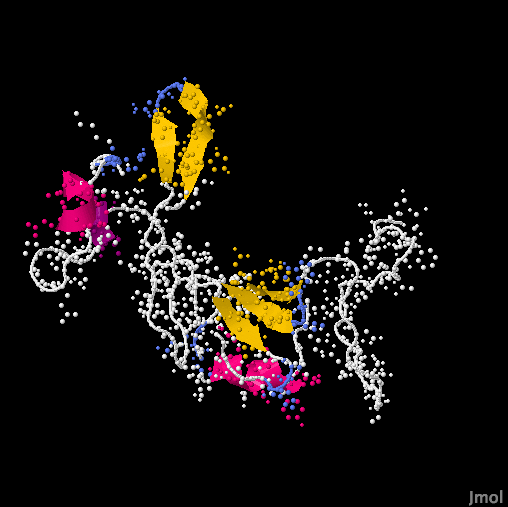
\includegraphics[width=.9\linewidth]{target_group_v2}
  \captionof{figure}{Target structure}
  \label{fig:test1}
\end{minipage}%
\begin{minipage}{.5\textwidth}
  \centering
  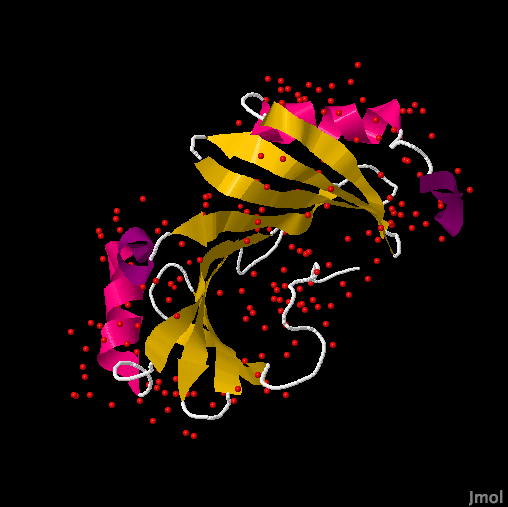
\includegraphics[width=.9\linewidth]{target_native}
  \captionof{figure}{Native structure}
  \label{fig:test2}
\end{minipage}
\end{figure}

\section{Results}



\subsection{Scores}
\begin{center}
    \begin{tabular}{ | l | l | l | p{2cm} |}
    \hline
      & Group1 & MULTICOM & MuFold \\ \hline
    TM-Score & 0.9971 & 0.9072 & 0.1985 \\ \hline
    RMSD & 0.23 & 1.666 & 14.978 \\
    \hline
    \end{tabular}
\end{center}

\section{Citations}

We thank the following tools and papers: \\\\




\end{document}


\end{document}
